\chapter{Results}
\label{cha:results}

Now that the inner workings of the algorithm have been explained we will continue with the 
results of the evaluation procedure. The aim here is to understand if the proposed algorithm
is working as intended, and see how it compares against some industry standard solutions.
In order to do so we will first explain our methodologies, then we will take a look at the loss
functions of the optimizer in order to verify that the optimization loop is working as intended.
Afterward we will move to the proper evaluation section where we will compare our solution
with a few industry standard using three key metrics (namely material used, optimization time, and printing
time). Finally we will move show a few real world printing tests to see how well the generated
support actually behaved when printed.

\section{Methodologies}

Before we start with our results we must state the methodologies. Those include the 3D models we used 
to evaluate our solution (the dataset), the ``Baseline Methods'' (i.e. the current industry standard
solution that we will compare our result with), and the Hardware and Software used to run the tests.

\subsection{3D Models}

Evaluating a support generation algorithm require of course the need to have some 3D models to evaluate 
the solution on. Since the research field of optimizing support structure generation for additive manufacturing
is quite niche, there is not a standard dataset that we can simply pick and use. Therefore we have manually
selected three models. We should note that those three models are not representative of the average object
printed by a regular user, this is because most 3D printing models are explicitly designed to be printed without
the need for supports, and would therefore be terrible testcases four our need. For this reasons we have 
explicitly ``charry piked'' models that require an heavy use of supports, so that we could better
appreciate the difference between the various approaches.
The three models we selected are a ``Dragon'' and a ``Candlestick'' taken from the ``printables'' online repository
and ``Armadillo'' taken from Stanford's 3D Scanning Repository.

\subsection{Baseline Methods}

Selecting our baselines methods was a bit challenging as there is no clear ``state of the art''
for what we are trying to do. The two papers that we have looked at in the \ref{cha:prev_literature}
chapter are not concerted with FDM 3D printing, and don't consider the necessary requirements of 
stiffness, making them not really suitable for our application. Furthermore their code is not publicly
available, We have even asked the authors access to the code for comparison use only
but they were unable to fulfill our request due to contractual obligation with industrial partners.
This left only with the options provided by the industry ``Normal'' and ``Tree'' supports (that we have
looked at in the \ref{cha:prev_literature} chapter).

\subsection{Hardware}

All runs have been conducted on an i7 14700HX laptop cpu with 64GB of ram.
The test have been executed while the laptop was fully charged, and connected to the power
plug, without any kind of power saving enabled.
The 3D printer used is an first generation Elegoo Century Carbon 3D printer using
Elegoo PLA as the material of choice.

\subsection{Software}

The test were run on Linux (NixOS 25.11 to be specific) and the code was 
written in Rust, and compiled in release mode without any specific compiler flag.
The rustc version was 1.93.1, and the toolchain used was the stable one.
The code was written to take advantage of multithreading, with the optimization
process regularly saturating all the CPU cores.

\subsection{Tests Number and Naming}

To reduce variability whe have have run our algorithm 5 times for each 
3D model for a total of 15 tests. In the case of the industry standard solutions we
instead only run once, as the variability of those is quite small if not zero.
In the case of the testcase ``Dragon'' we had to manually add some supports after
the one generated by the ``Tree'' algorithm failed to print four times in a row.
For this reason there are two different testcases for the dragon plus tree support combo.
Table \ref{tab:algorithm_maming} show the full list of the tests that have been performed,
with the algorithm and model associated with every test run.


\begin{table}[htbp]
  \centering
  \caption{Testcase list with algorithm and model used}
  \label{tab:algorithm_maming}
  \hspace{4pt}
  \begin{tabular}{lll}
    \toprule
    Test ID & Algorithm & Model \\
    \midrule
    ES1D & Evo Strut (ours) & Dragon \\
    ES2D & Evo Strut (ours) & Dragon \\
    ES3D & Evo Strut (ours) & Dragon \\
    ES4D & Evo Strut (ours) & Dragon \\
    ES5D & Evo Strut (ours) & Dragon \\
    ES1A & Evo Strut (ours) & Armadillo \\
    ES2A & Evo Strut (ours) & Armadillo \\
    ES3A & Evo Strut (ours) & Armadillo \\
    ES4A & Evo Strut (ours) & Armadillo \\
    ES5A & Evo Strut (ours) & Armadillo \\
    ES1C & Evo Strut (ours) & Candlestick \\
    ES2C & Evo Strut (ours) & Candlestick \\
    ES3C & Evo Strut (ours) & Candlestick \\
    ES4C & Evo Strut (ours) & Candlestick \\
    ES5C & Evo Strut (ours) & Candlestick \\
    \midrule
    TSD & Tree Supports & Dragon \\
    CTSD & Custom Tree Supports & Dragon \\
    TSA & Tree Supports & Armadillo \\
    TSC & Tree Supports & Candlestick \\
    \midrule
    NSD & Normal Supports & Dragon \\
    NSA & Normal Supports & Armadillo \\
    NSC & Normal Supports & Candlestick \\
    \bottomrule
  \end{tabular}
\end{table}


\section{Loss Function Trends}

In this section we will print the loss functions, in order to verify that the optimizer
is working properly, however unlike some more traditional optimization problems that have
a single loss function in our case we have many. Infant, as we detailed in chapter \ref{cha:support_opt_alg}
we have separated the optimization problem into three different stages, each of them with it's own
loss function, Furthermore, even within a single stage, we often use the divide and conquer approaches
where instead of solving an single optimization problem we have optimized many smaller one for a more efficient
computation. For example, in the case of the support structure optimization stage for testcase ES1D, the
support problem has been divided into seven different subproblems, and the resulting loss function of each
of the seven run, as well as the total can be seen in figure \ref{fig:individual_problems_loss}.
It should be noted that in the chart the $x$ axis representing the number of iterations has been normalized
in the range 0-1, since every run used a different number of iterations to converge.
We have a total of 45 of this type of graph (5 testcases $\times$ 3 models $\times$ 3 pipeline stages), and
those can be seen in the official github repository, however for in this thesis we decided to only put 
9 aggregates (\ref{fig:es_dragon_cpg} to \ref{fig:es_candlestick_sso}). In this set of aggregates graphs we have grouped
the optimizer run by model and pipeline stage. In every graph we can see the total loss function
of every one of the five runs, plus a single average loss function that gives the idea on how well
the algorithm is optimizing. This means, for example, that the ``Total'' line of graph \ref{fig:individual_problems_loss}
is the transparent blue line in graph \ref{fig:es_dragon_sso}.


\begin{figure}[h]
    \centering
    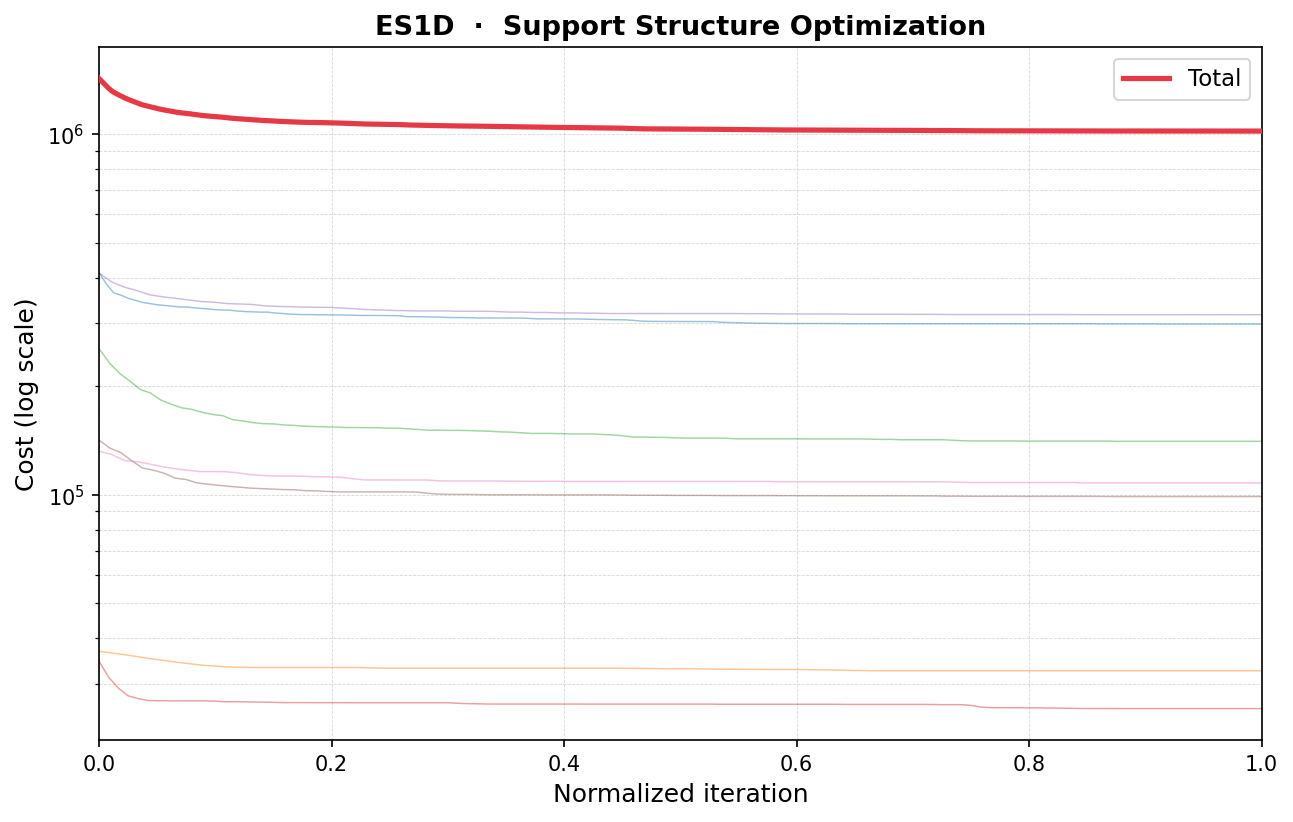
\includegraphics[width=0.5\textwidth]{images/ES1D_support_structure_optimization.png}
    \caption{Loss function of the support structure optimization stage for testcase ES1D}
    \label{fig:individual_problems_loss}
\end{figure}


Looking at all the loss functions we can note how the algorithm is performing quite well (at least
from the point of view of the loss function). 
The first thing that we can note when observing the threads, is that the loss
never degreases, this is of course to be expected given that all three of our optimizers use elitism
in their evolution process. Some of the graph (especially the one about the contact point optimization
stage) are particularly smooth, this both a symptom of the fact that there are a few averages/summations
smoothing out the process, and also of the fact that the first optimization stage is by far the easiest
and more linear of the three.
In some of the graph, we can see that all testcases from one to five at the end converge to a similar value
of the loss function, but on some others (most notably \ref{fig:es_dragon_sso} and \ref{fig:es_candlestick_cpg})
we can see that the different runs converge to different final values
for the loss function. This is almost certainty caused by the optimizer getting stuck in a local minimum
and not being able to further improve the loss, which is a pretty common scenario in most genetic algorithm and gradient
descent like optimizers. If anything our choice to use a three stages optimization problem is increasing
the likelihood of this type of scenario occurring, as every new stage can diverge from the ``optimal'' path
creating a cascade effect that can substantially vary the final output.
However we should not overstate the impact that this effect has on the quality of the solutions, 
even acknowledging that some of the testcases did not perform as well as others the overall thread
is still quite good, with the rate of improve decreasing over time, but still managing a substantial
improvement by the end of the run.



\begin{figure}[H]
    \centering
    \begin{minipage}{0.48\textwidth}
        \centering
        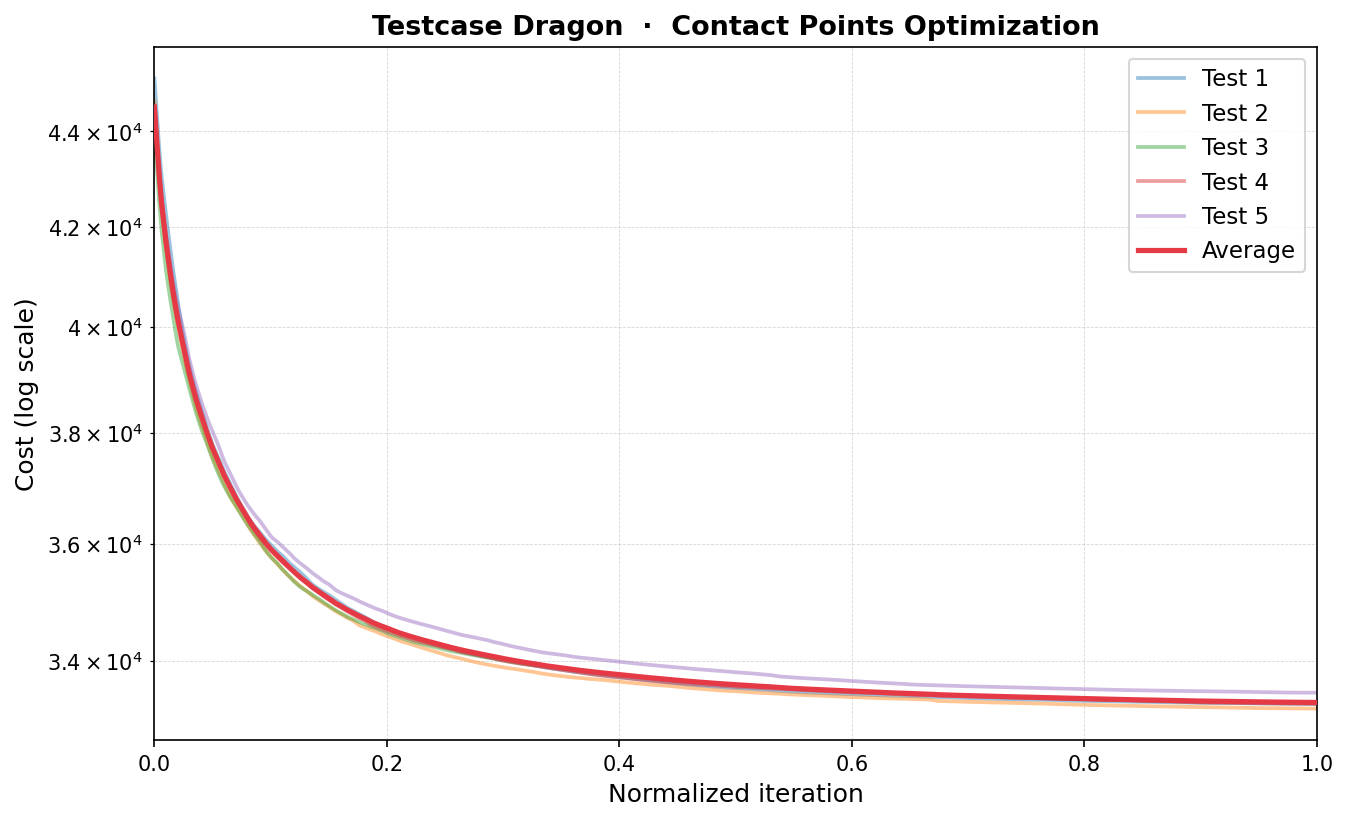
\includegraphics[width=\textwidth]{images/ES_Dragon_contact_points_optimization.png}
        \caption{Contact points optimization loss trend for the Dragon model}
        \label{fig:es_dragon_cpo}
    \end{minipage}
    \hfill
    \begin{minipage}{0.48\textwidth}
        \centering
        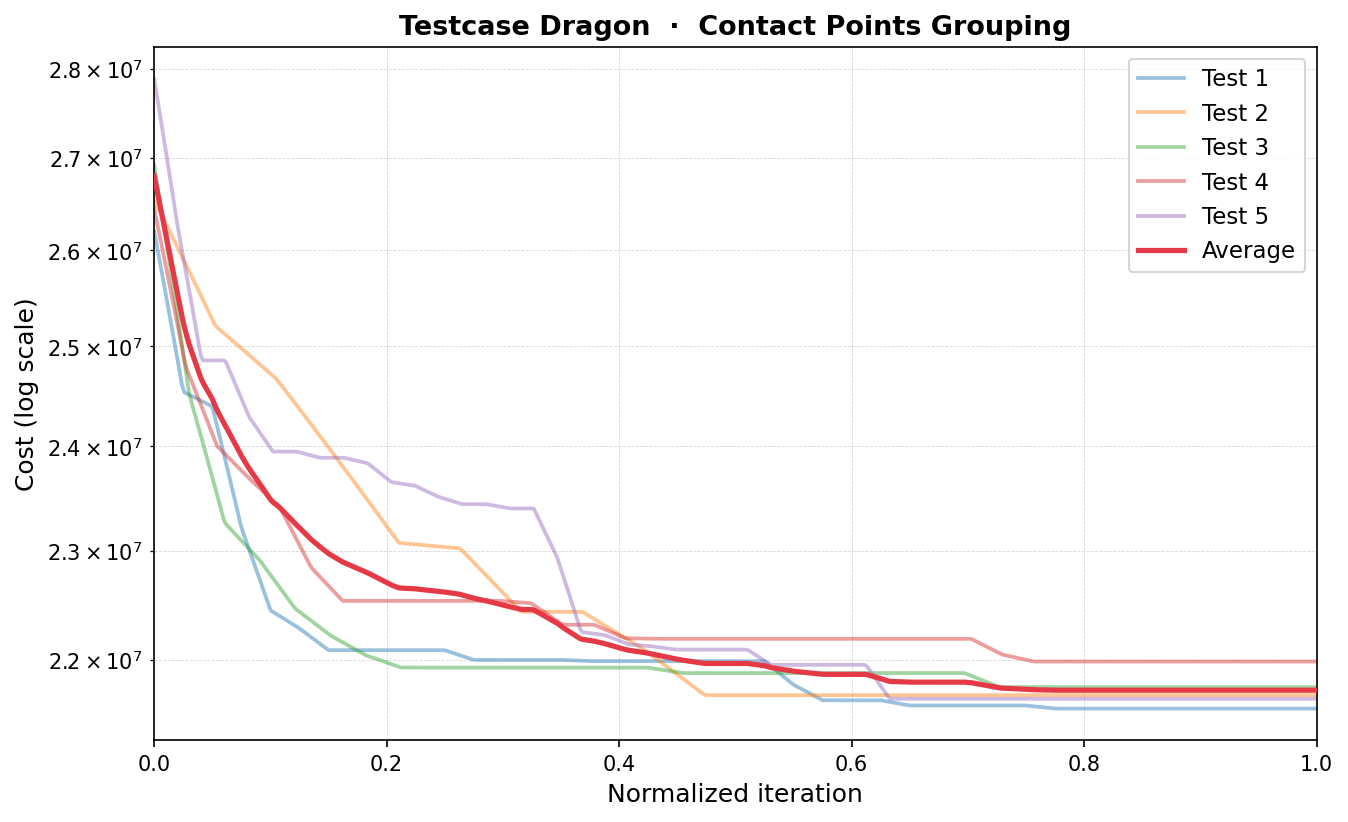
\includegraphics[width=\textwidth]{images/ES_Dragon_contact_points_grouping.png}
        \caption{Contact points grouping loss trend for the Dragon model}
        \label{fig:es_dragon_cpg}
    \end{minipage}
\end{figure}

\begin{figure}[H]
    \centering
    \begin{minipage}{0.48\textwidth}
        \centering
        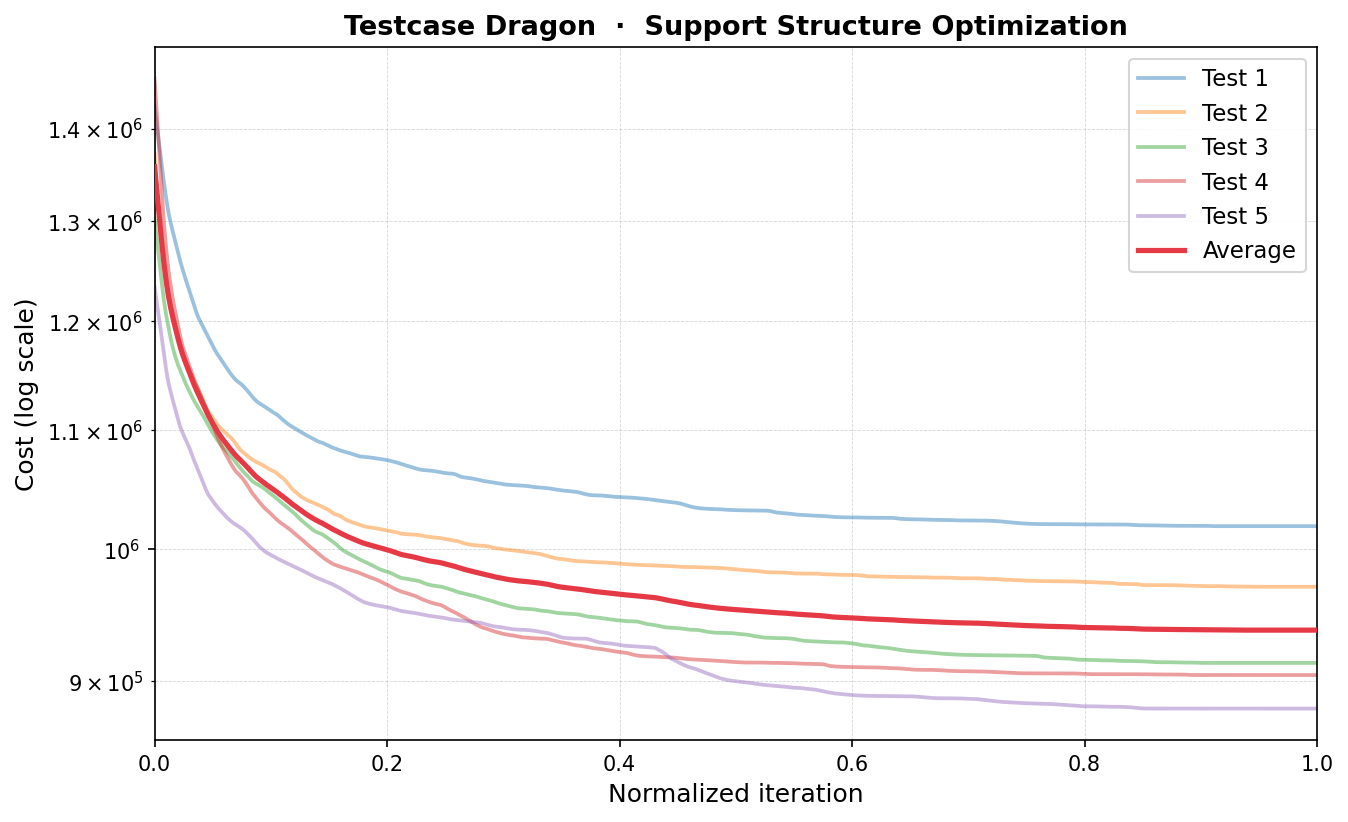
\includegraphics[width=\textwidth]{images/ES_Dragon_support_structure_optimization.png}
        \caption{Support structure optimization loss trend for the Dragon model}
        \label{fig:es_dragon_sso}
    \end{minipage}
    \hfill
    \begin{minipage}{0.48\textwidth}
        \centering
        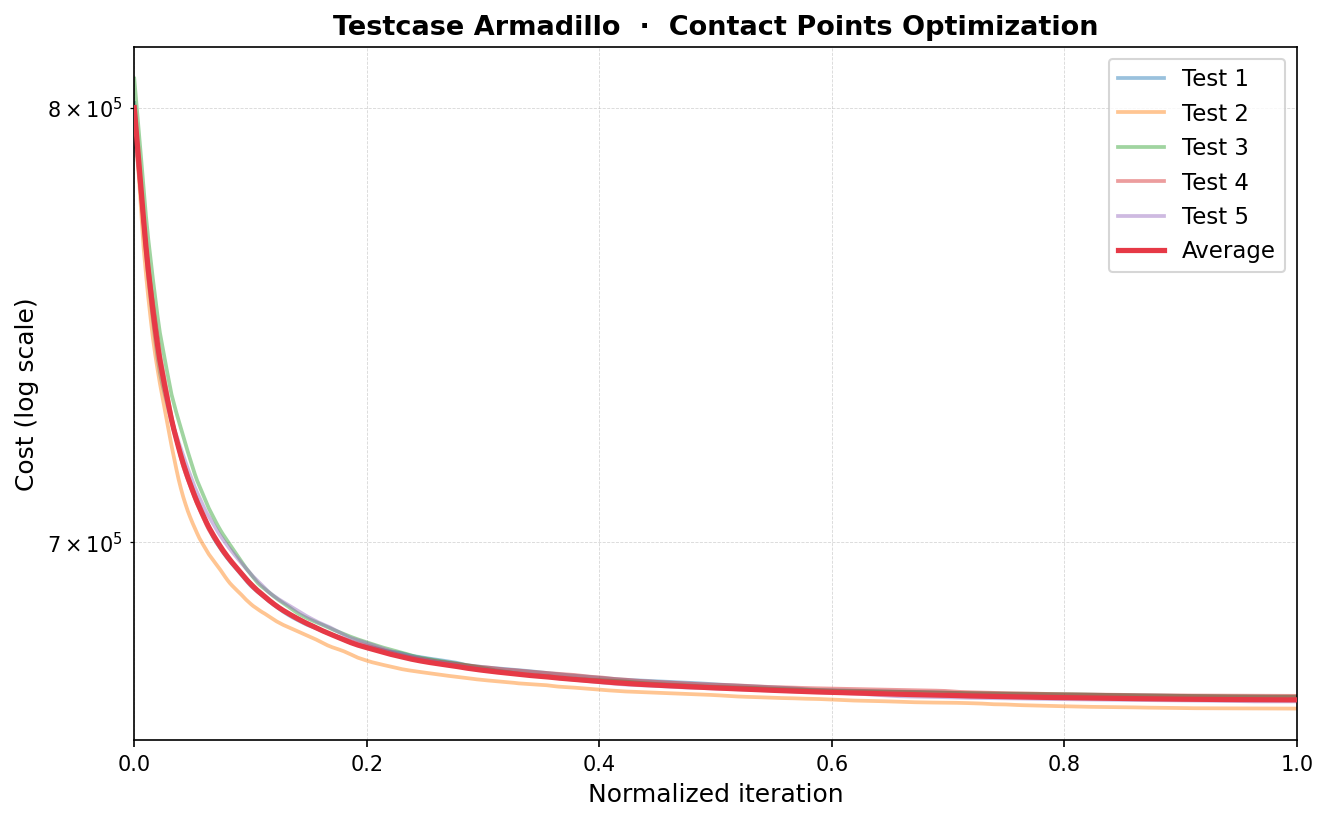
\includegraphics[width=\textwidth]{images/ES_Armadillo_contact_points_optimization.png}
        \caption{Contact points optimization loss trend for the Armadillo model}
        \label{fig:es_armadillo_cpo}
    \end{minipage}
\end{figure}

\begin{figure}[H]
    \centering
    \begin{minipage}{0.48\textwidth}
        \centering
        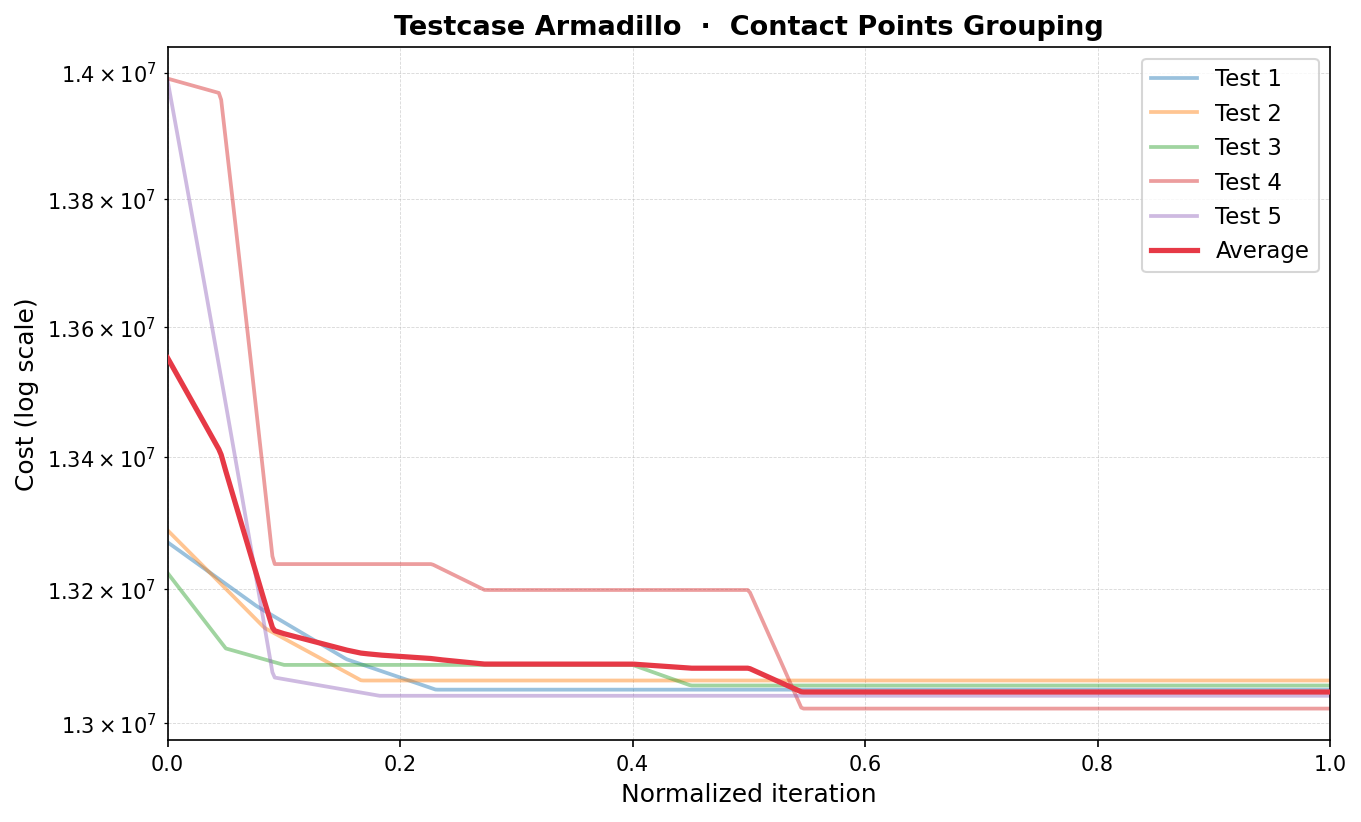
\includegraphics[width=\textwidth]{images/ES_Armadillo_contact_points_grouping.png}
        \caption{Contact points grouping loss trend for the Armadillo model}
        \label{fig:es_armadillo_cpg}
    \end{minipage}
    \hfill
    \begin{minipage}{0.48\textwidth}
        \centering
        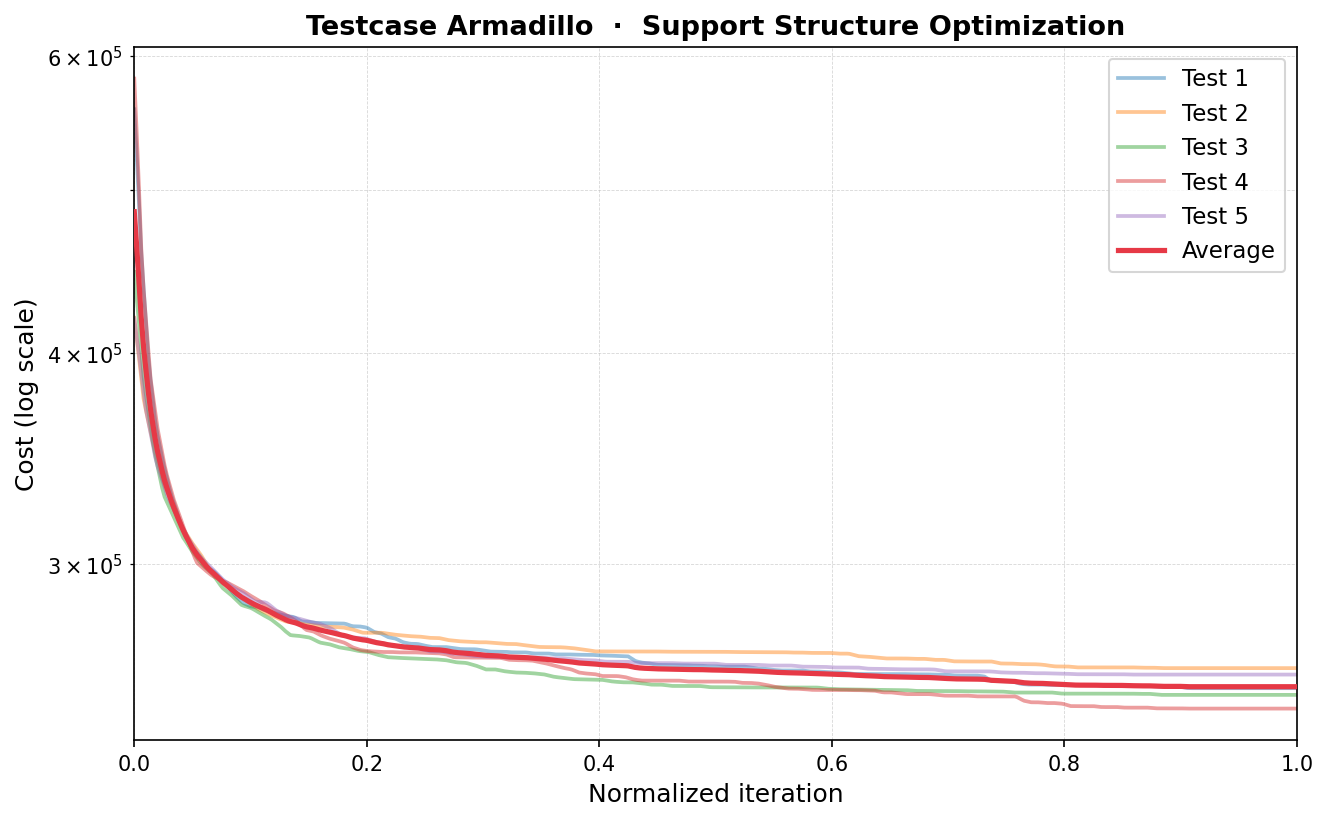
\includegraphics[width=\textwidth]{images/ES_Armadillo_support_structure_optimization.png}
        \caption{Support structure optimization loss trend for the Armadillo model}
        \label{fig:es_armadillo_sso}
    \end{minipage}
\end{figure}

\begin{figure}[H]
    \centering
    \begin{minipage}{0.48\textwidth}
        \centering
        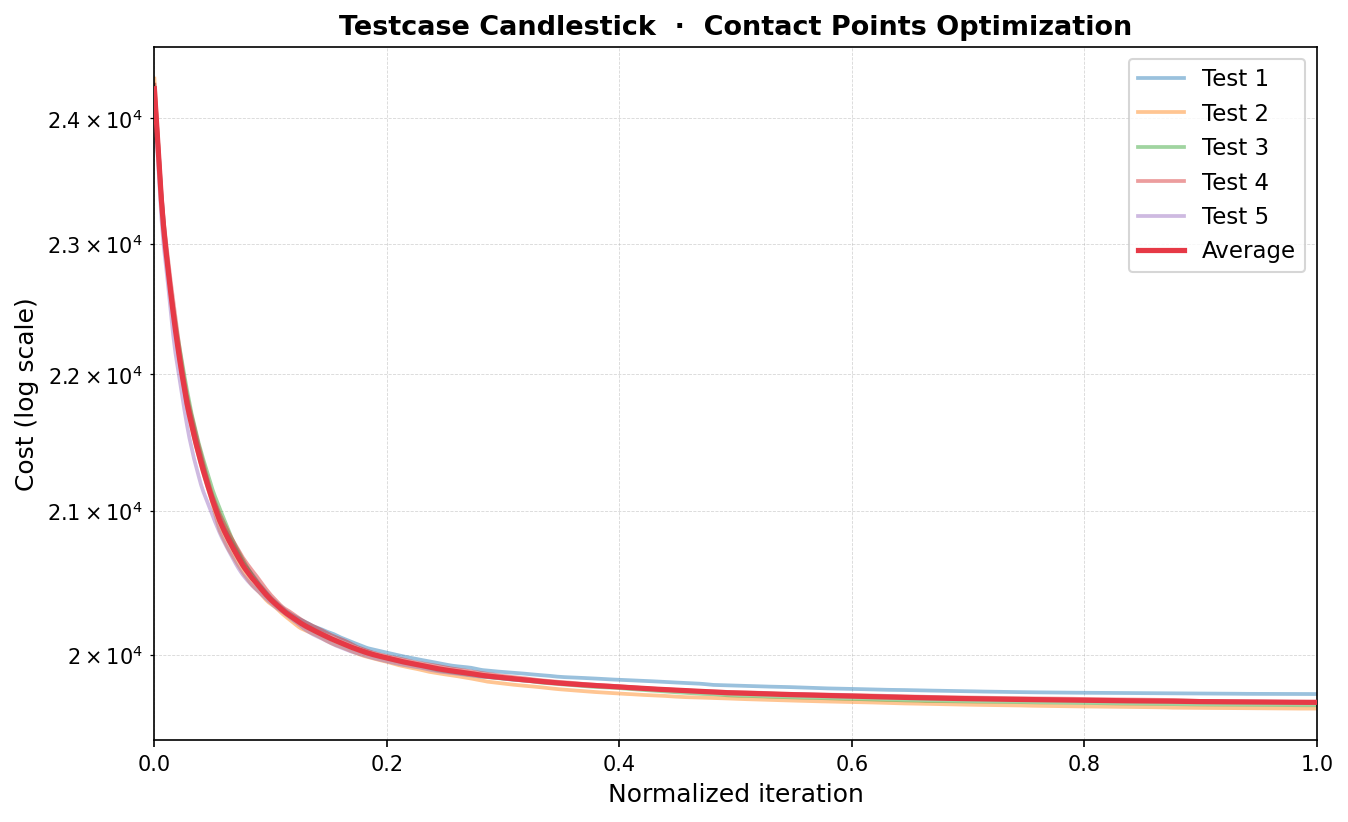
\includegraphics[width=\textwidth]{images/ES_Candlestick_contact_points_optimization.png}
        \caption{Contact points optimization loss trend for the Candlestick model}
        \label{fig:es_candlestick_cpo}
    \end{minipage}
    \hfill
    \begin{minipage}{0.48\textwidth}
        \centering
        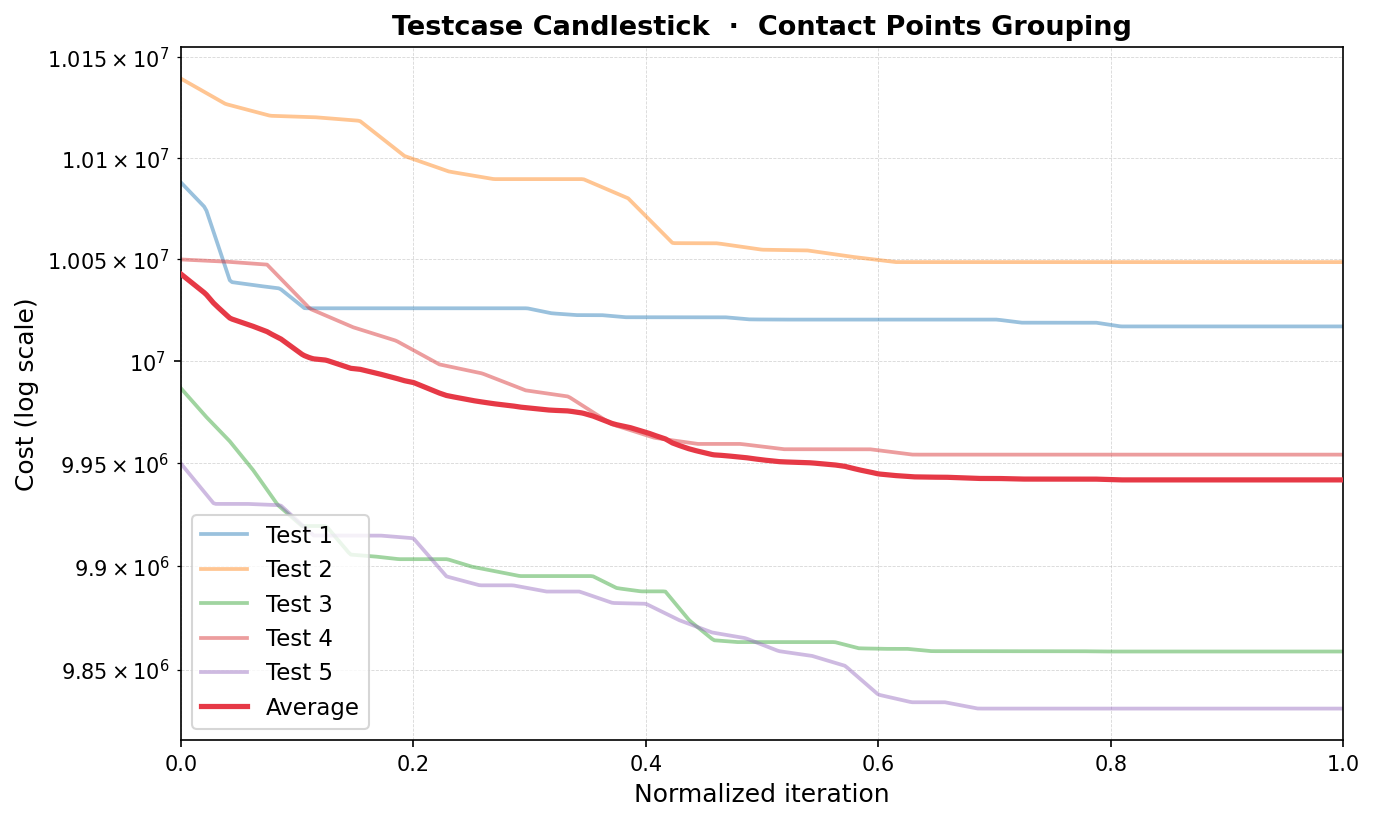
\includegraphics[width=\textwidth]{images/ES_Candlestick_contact_points_grouping.png}
        \caption{Contact points grouping loss trend for the Candlestick model}
        \label{fig:es_candlestick_cpg}
    \end{minipage}
\end{figure}

\begin{figure}[H]
    \centering
    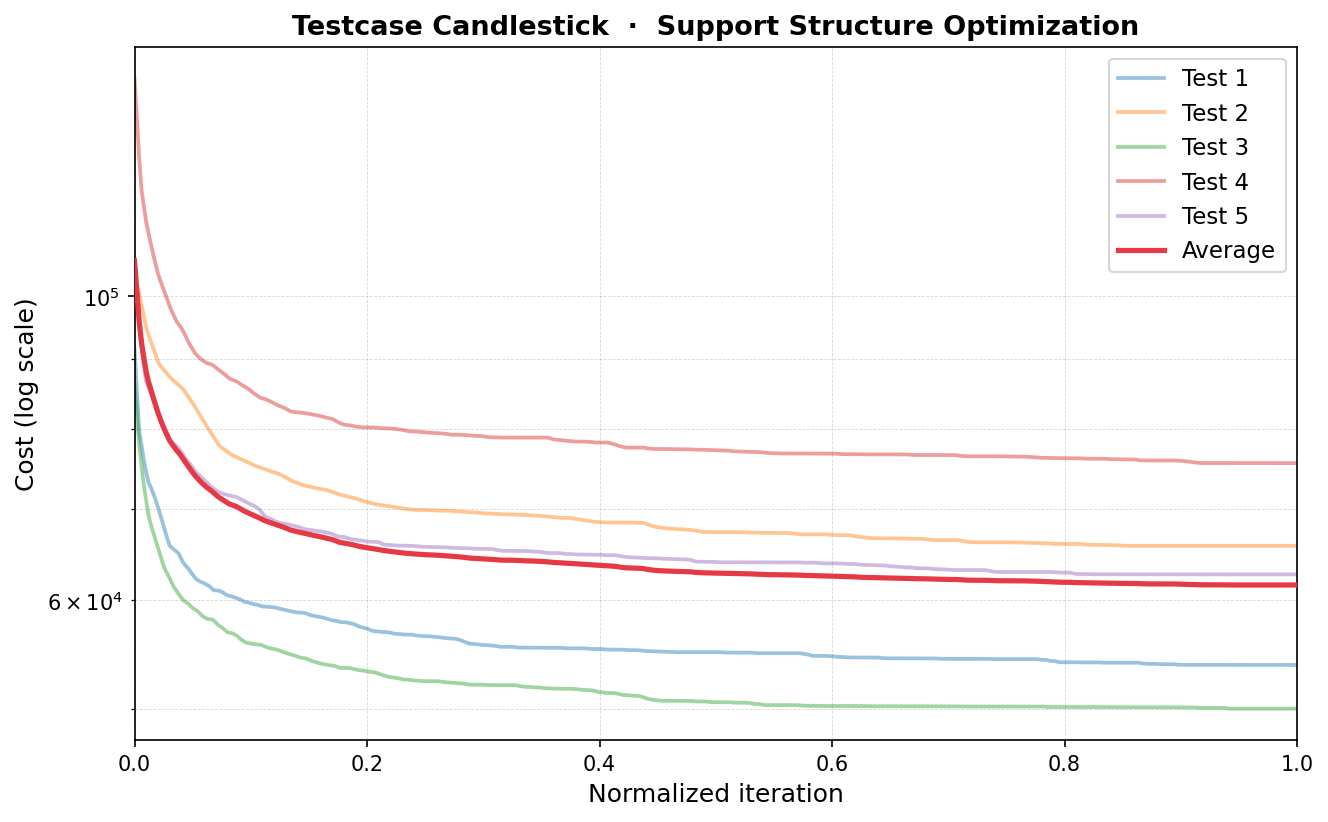
\includegraphics[width=0.5\textwidth]{images/ES_Candlestick_support_structure_optimization.png}
    \caption{Support structure optimization loss trend for the Candlestick model}
    \label{fig:es_candlestick_sso}
\end{figure}

\section{Reduction In material usage}

\section{Execution Time}

\section{Print Time}

\section{Print Tests}

